\subsection{WDM Subject}

We ultimately seek to design a target that will be heated to a WDM plasma using the OMEGA laser. The goal is to measure the stopping power of high energy protons through said WDM plasma. It is therefore crucial, that the target has a very well defined areal density ($\rho L$). This is accomplished through two ways. Firstly the targets are cylindrical such that the protons can probe the linear dimension whose length $L$ will be well characterized before the experiment. We choose cylindrical so that the circular dimension can still take advantage of the OMEGA's spherical laser geometry. Secondly, the target will be solid with a well characterized density $\rho$ before the experiment. The target will be heated isochorically, such that this density remains constant throughout the entire experiment.   

The isochoric heating process is done through x-ray attenuation. The OMEGA laser beams directly illuminate the circular surface of the target which will be coated with an x-ray conversion material. The x-ray generated from the heat will penetrate through the rest of the target material, heating it uniformly and isochorically. A basic schematic of the target design is shown in Figure \ref{fig:wdmTargetCartoon}. 

\begin{figure}[h!]
    \centering
    \includegraphics[scale=0.8]{Figures/wdmTargetCartoon.pdf}
    \caption[WDM Target Cartoon]{Basic cartoon of the WDM target design. The target is a cylindrical plug with some length $L$ and some diameter $D$. It is made up of some primary target material that will be heated to WDM and is coated with some x-ray conversion material that will generate x-rays when heated by the OMEGA laser.}
    \label{fig:wdmTargetCartoon}
\end{figure}

There are 5 primary variables that must be determined: the primary target material, the diameter of the primary target ($D$), the length of the primary target ($L$), the x-ray conversion material, and the thickness of the x-ray conversion coating ($t$). 

The primary target material is a fairly straightforward choice. The laser energy at OMEGA is limited and the solid target is fairly massive which means it is very likely that the WDM plasma will not be heated to temperatures high enough to fully ionize anything with $Z>2$. If the target $Z$ is too high, the resultant plasma will consist primarily of bound electrons which will act very similar to a cold target. In order to get results that are distinguishable from cold matter stopping, our target $Z$ must be as low as possible. This points to materials such as Li, Be, B, or C. While Li is the most ideal choice, it is also very difficult to work with and thus was not used in the experiments reported in this work.

Due to the limited energy issue previously discussed, both $D$ and $L$ should be minimized as much as possible to minimize the total mass of that target and thus maximize the final plasma temperature. However, both these dimensions cannot be arbitrarily small for two separate reasons. $L$ must be sufficiently large such that a significant amount of energy is lost $\Delta E$ by the protons probing the plasma. The uncertainty on $\Delta E$ is somewhat fixed around 50 keV by the systematic of the detectors and counting statistics. We therefore want $\Delta E \gg 50$ keV to ensure that our measurement is significant. In reality though, what we actually care about is the difference in energy loss between WDM plasmas and cold matter. This sets a much more stringent requirement that $|\Delta E_{WDM} - \Delta E_{cold}| \gg 50$ keV. Figure \ref{fig:wdmTeEstimation} shows these trade offs as a function of length for a Be target. 

\begin{figure}[!h]
    \centering
    \includegraphics[scale=0.7]{Figures/wdmTeEstimation.pdf}
    \caption[WDM Target Te vs Length]{Estimations for the target $T_e$ and the differences between warm and cold stopping as a function of the target length. As the target gets too long, the temperature decreases resulting in a smaller difference in the stopping power. All parameters were calculated for a Be plug of diameter 800 $\mu$m illuminated by 30 OMEGA laser beams, with an assumed x-ray conversion efficiency of 1\%.}
    \label{fig:wdmTeEstimation}
\end{figure}

As we can see in Figure \ref{fig:wdmTeEstimation}, the quantity that we intend to measure ($|\Delta E_{WDM} - \Delta E_{cold}|$) reaches a maximum at a length of approximately 300 $\mu$m. This is because as the target gets longer, the final $T_e$ gets smaller such as to bring the target closer to cold matter. In the limit where $T_e \xrightarrow{} 0$, the difference in stopping also goes to 0 because the WDM target is effectively cold matter. 

The diameter cannot be arbitrary small because of the heating mechanism. When the lasers illuminate the circular surface of the plug, a shock wave in launched inward toward the center of the plug. The density and temperature behind the shock-wave are difficult to characterize accurately and therefore are undesirable plasma properties to probe. To avoid this, we must probe the un-shocked region far before the shock can reach it. Figure \ref{fig:WDM_shock_cartoon} shows a cartoon of this requirement.

\begin{figure}[!h]
    \centering
    \includegraphics[scale=0.7]{Figures/WDM_shock_cartoon.pdf}
    \caption[WDM Target Shock Wave Timing Cartoon]{Cartoon of the shock wave traveling through the WDM target. The shocked region is depicted as a dark green and the un-shocked region is shown as a light green. For the experiment to be successful, protons can only go through the un-shocked region where the plasma properties are well known. }
    \label{fig:WDM_shock_cartoon}
\end{figure}

As seen in Figure \ref{fig:WDM_shock_cartoon}, the protons probe the target at an angle $\theta=12^{\circ}$. This is done for reasons that will be discussed in Section \ref{}. As a result, the protons probe radii between 0 to $(L/2)\sin\theta$. Meanwhile the shock-wave travels inward at some velocity similar to the sound speed $c_s$ of the material. This creates the requirement that:
%
\begin{equation}
    D \gg L \sin \theta + 2c_s \tau 
\end{equation}
%
where $\tau\sim 1.5$ns is the time between the lasers hitting the target and the protons leaving the target. The exact value of this requirement depends on many variables, but generally resolves to be of order 200-300 $\mu$m. 

The x-ray conversion material must be chosen based on the primary target material. The goal is to choose an x-ray energy whose attenuation length is roughly of order $D$. X-ray energies that attenuation lengths much lower than $D$ will result in a non-uniform temperature profile because the x-rays will not fully attenuate through the target. X-rays with much high attenuation lengths won't deposit a significant amount of energy into the target, decreasing the total efficiency. Figure \ref{fig:xrayAttenuation} shows the attenuation lengths as a function of x-ray energy for various low Z target materials.

Another thing to consider when choosing the x-ray conversion material is the x-ray Thomson Scattering backlighter material. The plasma must be characterized using x-ray Thomson Scattering which requires it's own x-ray source. The details of this are discussed later in Section \ref{sec:XRTS}. It is very important that the x-ray energies of the conversion material and the Thomson Scattering source are well separated from one another. Failure to do so makes interpretation of the x-ray Thomson Scattering data very difficult.

\begin{figure}[!h]
    \centering
    \includegraphics[scale=0.7]{Figures/xrayAttenuationLengths.pdf}
    \caption[X-ray Attenuation Lengths]{X-ray attenuation lengths for various low Z target materials. The blue, red, green, purple, and black curves correspond to a Li, Be, B, graphite, and diamond target respectively.}
    \label{fig:xrayAttenuation}
\end{figure}

\subsection{Proton Source Configuration}

In order to measure the stopping power, high energy protons must be generated to probe the WDM material. For this we use a D$^3$He backlighter located 1 mm away from the subject plasma. For our experiments the backlighter was a 18 atm 50/50 D$^3$He filled capsule. The nominal OD was 860 $\mu$m and the nominal shell thickness was 2.0 $\mu$m of SiO$_2$. These dimensions were chosen to ensure a sufficient proton yield for the experiments.

The proton backlighter and the subject target must be located along the axis of a TIM. This is so a WRF will measure protons that travel through the center of the WDM plasma. Ideally, the axial face of the target would face the WRF but (as shown in Figure \ref{fig:WDM_shock_cartoon}) there are compelling experimental reasons to compromise on this.

The source energy must be observed as well using another WRF. The energy of the protons emitted have been demonstrated to be symmetric meaning the placement of the secondary WRF is fairly arbitrary. If the experiment allows for additional WRFs, this assumption can be verified in-situ by simply fielding more WRFs in different positions.

\subsection{X-ray Thomson Scattering Configuration}
\label{sec:XRTS}

In order to properly interpret the results of the stopping power measurements, the WDM plasma needs to have it's ionization and temperature accurately characterized. This is done using X-ray Thomson Scattering. For this technique to work, x-rays need to scatter within the plasma volume at a well defined angle into an x-ray spectrometer. The characteristics of the scattered x-ray spectra gives information about the plasma characteristics.

To achieve this, a x-ray foil was placed onto a cone attached to the axial face of the WDM target. The cone serves two purposes; it's angle defines the scattering angle of the x-rays and also shields the spectrometer from the direct emission of the foil. A cartoon of this configuration is shown in Figure \ref{fig:wdmConeCartoon}.

\begin{figure}[h!]
    \centering
    \includegraphics[scale=0.7]{Figures/wdmConeCartoon.pdf}
    \caption[Carton of X-ray Thomson Scattering Configuration]{Cartoon of the X-ray Thomson Scattering configuration. Note that the cone (gold color) is hollow, allowing for x-rays to scattering back into the x-ray spectrometer.}
    \label{fig:wdmConeCartoon}
\end{figure}

As seen in Figure \ref{fig:wdmConeCartoon} the x-ray spectrometer sits behind the shield cone such that it cannot see x-rays directly emitted from the source foil. Because of it's role as an x-ray shield, the cone material must be made out of some high-Z material. Ideally this material will be chosen such that any x-ray emitted from it are far outside the energy range of the scattered x-ray spectra. In our experiments both Au and Ta were used. It should also be noted that the shield cone has a collimator where it contacts the primary target. This is to shield the spectrometer from x-rays that scatter in the shocked region of the plasma. This collimator must have some diameter $D_c$ less than $D$ by at least $2c_s\tau$. Like before, the exact value of 2$c_s\tau$ varies, but tends to be of order 100-200 $\mu$m. 

It should be noted that the proton source configuration and the x-ray Thomson Scattering configuration describe two distinct experiments. While it's not necessarily impossible to do both measurements at once, there are several obstacles that make attempting so undesirable. First of all, the proton source is a large source of Bremsstrahlung x-rays which would wash out the desired scattered x-ray spectra. Secondly, the shield cone effect the energy of the protons going through the target plasma. With some adjustments and very careful considerations a dual measurement may be possible, but was never attempted in this work.


\section{Beam Pointing}

\todo{If you have time, talk about how to configure the beam pointing}
